% Compile with: latexmk -xelatex Final_Hand_Gesture_Report_Team14.tex
\documentclass[10pt,twocolumn,a4paper]{article}

\usepackage[a4paper,top=0.72in,bottom=0.78in,left=0.66in,right=0.66in,
            columnsep=0.24in]{geometry}
\usepackage{fontspec}
\setmainfont{Latin Modern Roman}
\setsansfont{Latin Modern Sans}
\setmonofont{Latin Modern Mono}
% Use Microsoft JhengHei when available (Windows). Otherwise fall back to a CJK
% font that is present and embeddable on Linux. Note: Noto's variable-font .ttc
% releases break xdvipdfmx ("Invalid TTC index number"), so prefer the plain
% Droid Sans Fallback TTF, with Noto Sans CJK TC only as a last resort.
\IfFontExistsTF{Microsoft JhengHei}
  {\newfontfamily\zhfont{Microsoft JhengHei}}
  {\IfFontExistsTF{Droid Sans Fallback}
    {\newfontfamily\zhfont{Droid Sans Fallback}}
    {\newfontfamily\zhfont{Noto Sans CJK TC}}}
\usepackage{graphicx}
\usepackage{booktabs}
\usepackage{array}
\usepackage{amsmath,amssymb}
\usepackage{xcolor}
\usepackage{enumitem}
\usepackage[numbers,sort&compress]{natbib}
\usepackage{hyperref}
\usepackage{url}
\usepackage{fancyhdr}
\usepackage{caption}
\usepackage{subcaption}
\usepackage{tikz}
\usetikzlibrary{positioning,arrows.meta,calc}
\usepackage{flafter}
\usepackage{placeins}

\setlength{\parindent}{1em}
\setlength{\parskip}{0pt}
\setlength{\textfloatsep}{8pt plus 2pt minus 2pt}
\setlength{\floatsep}{7pt plus 2pt minus 2pt}
\setlength{\intextsep}{7pt plus 2pt minus 2pt}
\setlength{\abovecaptionskip}{4pt}
\setlength{\belowcaptionskip}{0pt}
\setlist[itemize]{leftmargin=*,topsep=2pt,itemsep=1pt,parsep=0pt}
\setlist[enumerate]{leftmargin=*,topsep=2pt,itemsep=1pt,parsep=0pt}
\captionsetup{font=small,labelfont=bf}

\definecolor{linkblue}{RGB}{22,73,132}
\definecolor{boxgray}{RGB}{245,247,250}
\hypersetup{
  colorlinks=true,
  linkcolor=linkblue,
  citecolor=linkblue,
  urlcolor=linkblue
}

\pagestyle{fancy}
\fancyhf{}
\fancyhead[L]{Multimedia Final Project}
\fancyhead[R]{Team 14}
\fancyfoot[C]{\thepage}
\renewcommand{\headrulewidth}{0.3pt}
\setlength{\headheight}{13pt}

\newcommand{\ProjectRepository}{https://github.com/xxjustintwxx/Multimedia_Final_Project}
\newcommand{\codepath}[1]{%
  \href{\ProjectRepository/blob/main/#1}{\nolinkurl{#1}}%
}
\newcommand{\evidence}[1]{\textsuperscript{\scriptsize[\hyperref[ev:#1]{#1}]}}
\newcommand{\result}[2]{#1\evidence{#2}}
\newcommand{\MainTextEndsHere}{\label{main-text-end}\clearpage}
\newcommand{\modelbox}[1]{%
  \colorbox{boxgray}{\parbox[c][0.72in][c]{0.22\textwidth}{\centering #1}}%
}

\title{\vspace{-1.4em}\textbf{Hand Gesture Classification on Edge Devices}}
\author{Team 14\\[2pt]
  {\zhfont 王昱閔 \quad 王辰竹 \quad 羅詠璿}}
\date{}

\begin{document}
\maketitle
\thispagestyle{fancy}

\begin{abstract}
We present a compact multimodal hand-gesture classifier for edge deployment.
The model receives only a cropped RGB hand image and 21 MediaPipe landmarks,
then predicts one of five command gestures or rejects the input as N/A. A
depthwise-separable convolutional branch captures appearance, while a
landmark multilayer perceptron captures hand geometry. Their features are
fused and followed by confidence-based rejection calibrated for an asymmetric
evaluation rule in which a false trigger is penalized twice as heavily as a
correct command is rewarded. The final network contains
\result{36,039}{VERIFY} trainable parameters. Its tensors occupy
\result{0.142 MiB}{VERIFY}, while the submitted PyTorch checkpoint occupies
\result{0.168 MiB}{VERIFY}. The best reported validation accuracy is
\result{96.75\%}{PROG}, and the stronger of two leaderboard submissions
obtained a pre-presentation subtotal of \result{81.4/90}{PRES}.
\end{abstract}

\section{Introduction}
\label{sec:introduction}

Touch-free gesture interfaces must recognize intended commands while avoiding
activation on ordinary hand poses. This requirement is especially important
on edge devices, where models must also remain compact and operate without
cloud inference. The course challenge fixes the upstream MediaPipe
preprocessor and permits the downstream classifier to receive only a cropped
RGB hand image and 21 hand landmarks~\cite{courseSpec,zhang2020mediapipehands}.

The task uses five valid commands---fist, like, OK, one, and palm---and maps
every other accepted one-hand pose to N/A. Its scoring rule gives one point
for a correct target prediction but subtracts two points for a false trigger
~\cite{courseSpec}. This asymmetry changes the design objective: maximizing
closed-set accuracy alone is insufficient, because uncertain samples should
often be rejected.

Our main contributions are:
\begin{itemize}
  \item a dual-stream model combining visual appearance and landmark geometry
        within a small parameter budget;
  \item a three-stage training procedure consisting of image pretraining,
        joint multimodal optimization, and scoring-aware calibration; and
  \item a conservative inference policy combining neural N/A prediction,
        confidence and margin gates, and landmark validity checking.
\end{itemize}

\section{Task and Evaluation}
\label{sec:task}

\subsection{Inputs and label space}

The deployed function follows the required
\texttt{predict(cropped\_img, landmarks)} interface
\evidence{INFER}. The image is resized to
\result{$64\times64$}{INFER} RGB pixels and normalized channel-wise from
$[0,1]$ to $[-1,1]$. The \result{21}{SPEC} crop-relative $(x,y)$ landmarks are
flattened into a \result{42}{INFER}-dimensional vector. The output mapping is
shown in Table~\ref{tab:classes}. Full-frame images are prohibited
~\cite{courseSpec}.

\begin{table}[!b]
  \centering
  \caption{Output label mapping used by the submitted inference code.}
  \label{tab:classes}
  \small
  \begin{tabular}{cl@{\qquad}cl}
    \toprule
    ID & Label & ID & Label \\
    \midrule
    0 & N/A & 3 & OK \\
    1 & fist & 4 & one \\
    2 & like & 5 & palm \\
    \bottomrule
  \end{tabular}
\end{table}

\subsection{Scoring rule}

The official evaluation allocates 30 points to model size, 20 to HaGRIDv2
performance, 40 to real-world robustness, and 30 to presentation
~\cite{courseSpec}. For a model no larger than 10 MB, the size score is
\begin{equation}
S_{\mathrm{size}}=(10-\mathrm{size}_{\mathrm{MB}})\times3.
\end{equation}
Both performance sets use the raw contribution
\begin{equation}
s_i =
\begin{cases}
  +1, & \text{correct target command},\\
  -2, & \text{false trigger},\\
  0,  & \text{N/A output}.
\end{cases}
\end{equation}
The robustness set contains 50 N/A interference images and 50 target images
~\cite{courseSpec}. Since one false trigger cancels two correct commands, we
optimize checkpoint selection and calibration with this scoring function in
addition to reporting accuracy.

\section{Related Work}
\label{sec:related-work}

MediaPipe Hands combines a palm detector and a landmark estimator for
real-time on-device hand tracking~\cite{zhang2020mediapipehands}. Its landmark
representation provides geometric information that is less dependent on
texture and illumination than RGB appearance alone. HaGRIDv2 is a large-scale
gesture dataset containing static, dynamic, and no-gesture examples
~\cite{nuzhdin2024hagridv2}. Our classifier uses its 512-pixel release while
following the challenge-specific target and N/A mapping.

To reduce computation, the image encoder uses depthwise-separable
convolutions, a factorization used by MobileNets to replace a standard spatial
convolution with depthwise and pointwise operations~\cite{howard2017mobilenets}.
The proposed network is task-specific and trained from scratch; it does not
use a gesture-recognition pretrained model.

\section{Proposed Method}
\label{sec:method}

\subsection{Dual-stream architecture}

\begin{figure*}[t]
  \centering
  \resizebox{\textwidth}{!}{%
  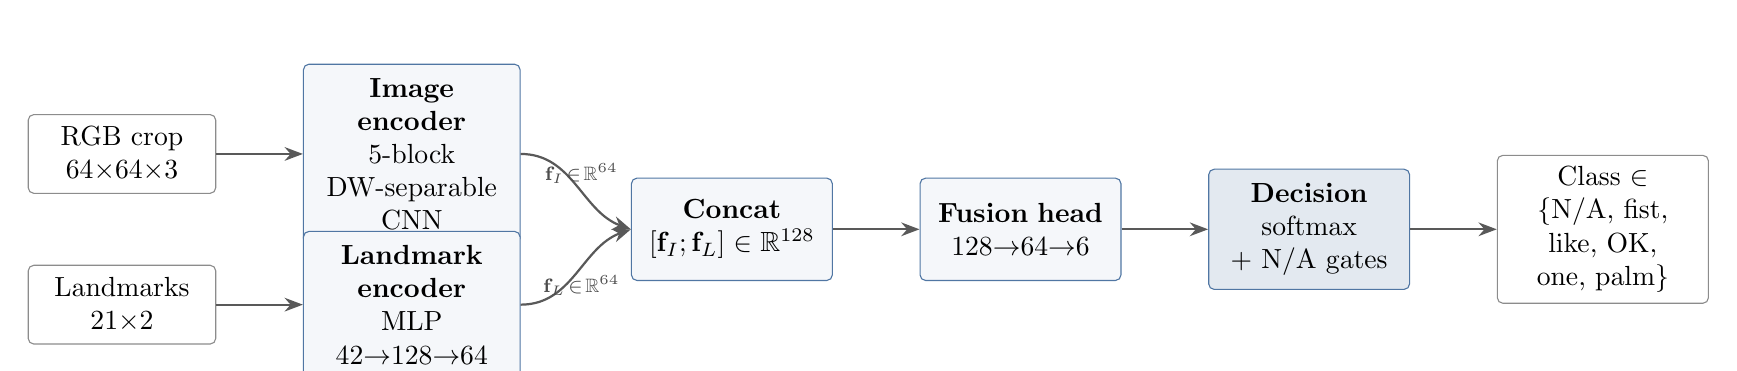
\begin{tikzpicture}[
      >=Stealth,
      node distance=8mm and 11mm,
      io/.style   ={rounded corners=2pt, draw=black!45, fill=white,
                    align=center, inner sep=4pt, minimum height=10mm,
                    text width=21mm},
      enc/.style  ={rounded corners=2pt, draw=linkblue!75, fill=boxgray,
                    align=center, inner sep=5pt, minimum height=13mm,
                    text width=24mm},
      op/.style   ={rounded corners=2pt, draw=linkblue!75, fill=boxgray,
                    align=center, inner sep=5pt, minimum height=13mm,
                    text width=22mm},
      dec/.style  ={rounded corners=2pt, draw=linkblue!75, fill=linkblue!12,
                    align=center, inner sep=5pt, minimum height=13mm,
                    text width=22mm},
      arr/.style  ={->, thick, draw=black!65},
      lbl/.style  ={font=\scriptsize, text=black!70, inner sep=2pt}
    ]
    % --- inputs ---
    \node[io] (img) {RGB crop\\$64{\times}64{\times}3$};
    \node[io, below=9mm of img] (lm) {Landmarks\\$21{\times}2$};
    % --- encoders ---
    \node[enc, right=of img] (cnn)
      {\textbf{Image encoder}\\5-block\\DW-separable CNN};
    \node[enc, right=of lm] (mlp)
      {\textbf{Landmark encoder}\\MLP\\$42{\to}128{\to}64$};
    % --- fusion / decision chain (centred between the two encoders) ---
    \path (cnn.east) -- (mlp.east) coordinate[midway] (mid);
    \node[op,  right=14mm of mid] (cat)
      {\textbf{Concat}\\$[\mathbf{f}_I;\mathbf{f}_L]\in\mathbb{R}^{128}$};
    \node[op,  right=of cat] (fuse) {\textbf{Fusion head}\\$128{\to}64{\to}6$};
    \node[dec, right=of fuse] (dec) {\textbf{Decision}\\softmax\\$+$ N/A gates};
    \node[io,  right=of dec, text width=24mm] (out)
      {Class $\in\{$N/A, fist,\\like, OK, one, palm$\}$};
    % --- arrows ---
    \draw[arr] (img) -- (cnn);
    \draw[arr] (lm)  -- (mlp);
    \draw[arr] (cnn.east) to[out=0,in=160]
      node[lbl, above, pos=0.55]{$\mathbf{f}_I\!\in\!\mathbb{R}^{64}$} (cat.west);
    \draw[arr] (mlp.east) to[out=0,in=200]
      node[lbl, below, pos=0.55]{$\mathbf{f}_L\!\in\!\mathbb{R}^{64}$} (cat.west);
    \draw[arr] (cat)  -- (fuse);
    \draw[arr] (fuse) -- (dec);
    \draw[arr] (dec)  -- (out);
  \end{tikzpicture}}
  \caption{Overview of the dual-stream classifier. A MediaPipe-cropped RGB hand
  image and 21 crop-relative landmarks are encoded by two independent branches,
  each producing a 64-dimensional descriptor. The descriptors are concatenated
  into a 128-dimensional multimodal feature, mapped to six logits by the fusion
  head, and converted to a final label by the softmax and N/A-rejection gates.}
  \label{fig:architecture}
\end{figure*}

Figure~\ref{fig:architecture} summarizes the model. The RGB crop and landmark
vector are encoded independently, producing two 64-dimensional descriptors.
These descriptors are concatenated into a 128-dimensional multimodal feature,
which is classified into six logits. The image branch contains
\result{13,249}{VERIFY} trainable parameters, the landmark branch contains
\result{14,144}{VERIFY}, and the fusion head contains
\result{8,646}{VERIFY}. This division gives both modalities comparable model
capacity while keeping the complete network small.

\subsection{Image branch}

The image branch contains five depthwise-separable blocks. For an input with
$C$ channels, the $3\times3$ depthwise convolution uses $C$ groups and filters
each channel independently. A $1\times1$ pointwise convolution then mixes
information across channels and changes the channel count. Each operation is
followed by batch normalization and ReLU
~\cite{ioffe2015batchnorm}. This factorization replaces a dense spatial
convolution while preserving its local receptive field.

A central design decision keeps the model far smaller than typical
submissions: we reuse only the depthwise-separable \emph{building block}
introduced by MobileNet~\cite{howard2017mobilenets}, rather than an entire
MobileNet backbone. A complete MobileNetV2 or MobileNetV3 image encoder holds
on the order of millions of parameters---roughly 3.4\,M and 2.5\,M for
MobileNetV2 and MobileNetV3-Small, respectively---and
is usually deployed by fine-tuning ImageNet-pretrained
weights~\cite{sandler2018mobilenetv2,howard2019mobilenetv3}. In contrast, our
image encoder stacks only five such blocks and is trained from scratch on the
gesture data (Section~\ref{sec:training}), so it contains just
\result{13{,}249}{VERIFY} parameters---about two orders of magnitude fewer than
a full backbone, as summarized in Table~\ref{tab:size-compare}. Two factors
make this reduced capacity sufficient: the hand crop is already tightly
localized by the fixed MediaPipe stage, and only six coarse classes must be
separated. This choice, rather than post-hoc compression, is the primary reason
the complete network occupies under 0.2~MiB instead of the several megabytes
typical of a fine-tuned backbone, which directly raises the size component of
the official score.

\begin{table}[t]
  \centering
  \caption{Parameter-count comparison between our from-scratch image encoder
  and standard MobileNet image backbones. MobileNet counts are the published
  ImageNet encoder sizes~\cite{sandler2018mobilenetv2,howard2019mobilenetv3};
  ours are recomputed from the model definition\evidence{VERIFY}.}
  \label{tab:size-compare}
  \small
  \setlength{\tabcolsep}{5pt}
  \begin{tabular}{lr}
    \toprule
    Image encoder & Parameters \\
    \midrule
    MobileNetV2 (full backbone)        & $\sim$3{,}400{,}000 \\
    MobileNetV3-Small (full backbone)  & $\sim$2{,}500{,}000 \\
    \textbf{Ours} (5 DW-sep blocks, from scratch) & \textbf{13{,}249} \\
    \midrule
    \textbf{Ours} (full dual-stream model)        & \textbf{36{,}039} \\
    \bottomrule
  \end{tabular}
\end{table}

Table~\ref{tab:image-branch} gives the complete tensor progression. The first
three blocks use stride two and reduce the spatial resolution from
\result{$64{\times}64$ to $8{\times}8$}{ARCH}; Blocks 4 and 5 refine the
features without further downsampling. Adaptive global average pooling
averages each of the final 64 feature maps over its $8\times8$ spatial grid,
yielding one scalar per channel and therefore a
\result{64-dimensional}{ARCH} image descriptor.

\begin{table}[t]
  \centering
  \caption{Detailed image-branch architecture. Every block follows
  DWConv--BN--ReLU--PWConv--BN--ReLU.}
  \label{tab:image-branch}
  \small
  \begin{tabular}{lccc}
    \toprule
    Layer & Input tensor & Output tensor & Stride \\
    \midrule
    Block 1 & $64{\times}64{\times}3$  & $32{\times}32{\times}16$ & 2 \\
    Block 2 & $32{\times}32{\times}16$ & $16{\times}16{\times}32$ & 2 \\
    Block 3 & $16{\times}16{\times}32$ & $8{\times}8{\times}64$   & 2 \\
    Block 4 & $8{\times}8{\times}64$   & $8{\times}8{\times}64$   & 1 \\
    Block 5 & $8{\times}8{\times}64$   & $8{\times}8{\times}64$   & 1 \\
    GAP     & $8{\times}8{\times}64$   & $64$                     & -- \\
    \bottomrule
  \end{tabular}
\end{table}

The branch is also inexpensive to evaluate. Summing the multiply--accumulate
operations of every layer in Table~\ref{tab:image-branch} gives
\result{$\approx$1.0\,M}{VERIFY} MACs (about 2.0\,MFLOPs) for one forward pass,
of which the image branch accounts for \result{98\%}{VERIFY}; the landmark and
fusion paths together contribute only about 22\,k MACs. The model is therefore
cheap to run per frame in addition to being small to store, which matters for
the edge setting where compute, not just disk size, is constrained.

\subsection{Landmark branch and fusion}

The landmark input preserves the order of the 21 MediaPipe points. Its
crop-relative $(x,y)$ coordinates are flattened in landmark order, producing
42 values. The landmark branch first projects
\result{$42{\to}128$}{ARCH}, applies batch normalization and ReLU, then
projects \result{$128{\to}64$}{ARCH} followed by another normalization and
ReLU. Unlike the image branch, this branch operates directly on finger and
palm geometry and is unaffected by crop texture or color.

Let $\mathbf{f}_{I}\in\mathbb{R}^{64}$ and
$\mathbf{f}_{L}\in\mathbb{R}^{64}$ denote the image and landmark descriptors.
Fusion is performed by direct concatenation,
\begin{equation}
\mathbf{f}=[\mathbf{f}_{I};\mathbf{f}_{L}]\in\mathbb{R}^{128}.
\end{equation}
The fusion head applies a \result{$128{\to}64$}{ARCH} linear layer and ReLU,
then \result{0.3}{ARCH} dropout during training. A final
\result{$64{\to}6$}{ARCH} layer produces one logit for N/A and one for each
target gesture. Softmax is applied only during evaluation and inference to
convert these logits into class probabilities.

\subsection{Conservative N/A rejection}

The deployed decision procedure contains three safeguards
\evidence{INFER}. Before running the network, it computes the horizontal and
vertical span of the 21 crop-relative landmarks. If the larger span is below
\result{0.05}{INFER}, all points have collapsed into a very small region and
the sample is immediately rejected as N/A. For a valid sample, the image and
landmarks pass through the two branches and softmax produces six
probabilities. If the highest-probability class is already class 0, the model
returns N/A directly. Otherwise, let $p_1$ be the highest non-N/A prediction
and $p_2$ the runner-up probability. The sample is rejected when
\begin{equation}
p_1 < \tau_c \quad \text{or} \quad p_1-p_2 < \tau_m .
\end{equation}
Calibration selected $\tau_c=\result{0.95}{CAL}$ and
$\tau_m=\result{0.00}{CAL}$. Therefore, the final deployed sequence is:
landmark validity check, six-class neural prediction, direct neural N/A
decision, and finally the 0.95 confidence gate, as shown in
Figure~\ref{fig:na-flow}. The margin condition remains
implemented for reproducibility and future recalibration, but a zero threshold
means it does not reject additional samples in the submitted configuration.

\begin{figure}[t]
  \centering
  \resizebox{0.95\columnwidth}{!}{%
  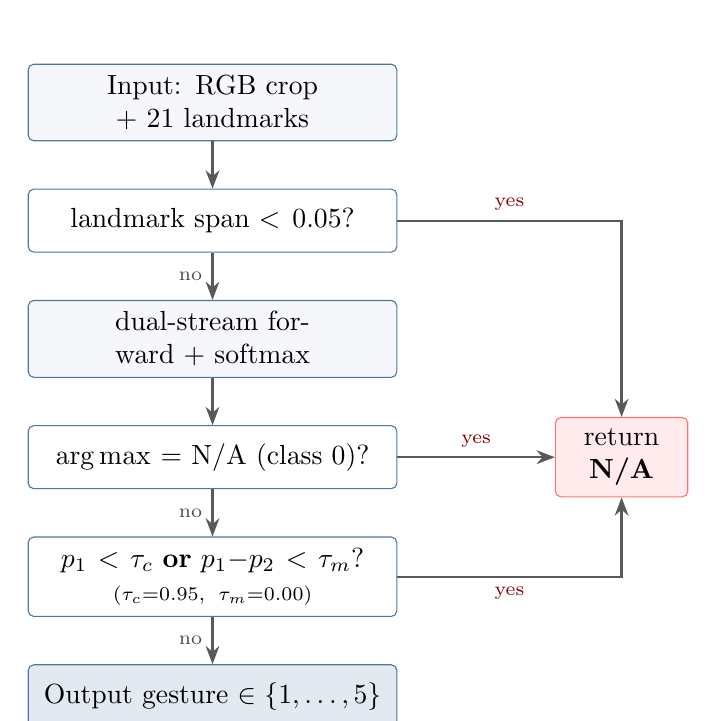
\begin{tikzpicture}[
      >=Stealth, node distance=6mm,
      proc/.style={rounded corners=2pt, draw=linkblue!75, fill=boxgray,
                   align=center, inner sep=4pt, text width=44mm,
                   minimum height=8mm},
      test/.style={rounded corners=2pt, draw=linkblue!75, fill=white,
                   align=center, inner sep=4pt, text width=44mm,
                   minimum height=8mm},
      na/.style={rounded corners=2pt, draw=red!55, fill=red!8,
                 align=center, inner sep=4pt, text width=14mm,
                 minimum height=9mm},
      term/.style={rounded corners=2pt, draw=linkblue!75, fill=linkblue!12,
                  align=center, inner sep=4pt, text width=44mm,
                  minimum height=8mm},
      arr/.style={->, thick, draw=black!65},
      yes/.style={font=\scriptsize, text=red!55!black},
      no/.style={font=\scriptsize, text=black!70}
    ]
    \node[proc] (in) {Input: RGB crop $+$ 21 landmarks};
    \node[test, below=of in]  (g1)  {landmark span $<0.05$?};
    \node[proc, below=of g1]  (net) {dual-stream forward $+$ softmax};
    \node[test, below=of net] (g2)  {$\arg\max=$ N/A (class 0)?};
    \node[test, below=of g2]  (g3)  {$p_1<\tau_c$ \textbf{or}
                                     $p_1{-}p_2<\tau_m$?\\
                                     {\scriptsize($\tau_c{=}0.95,\ \tau_m{=}0.00$)}};
    \node[term, below=of g3]  (out) {Output gesture $\in\{1,\dots,5\}$};
    \node[na, right=20mm of g2] (na) {return\\\textbf{N/A}};
    % pass (no) path down the centre
    \draw[arr] (in) -- (g1);
    \draw[arr] (g1)  -- node[no,left]{no} (net);
    \draw[arr] (net) -- (g2);
    \draw[arr] (g2)  -- node[no,left]{no} (g3);
    \draw[arr] (g3)  -- node[no,left]{no} (out);
    % reject (yes) paths to the N/A sink
    \draw[arr] (g1.east) -| node[yes,pos=0.25,above]{yes} (na.north);
    \draw[arr] (g2.east) -- node[yes,above]{yes} (na.west);
    \draw[arr] (g3.east) -| node[yes,pos=0.25,below]{yes} (na.south);
  \end{tikzpicture}}
  \caption{Deployed N/A-rejection decision flow~\evidence{INFER}. A sample is
  rejected as N/A if the landmarks collapse, if the network's top class is N/A,
  or if it fails the confidence gate; otherwise the predicted gesture is
  returned. The margin term is inactive at $\tau_m{=}0.00$.}
  \label{fig:na-flow}
\end{figure}

\section{Dataset and Preprocessing}
\label{sec:data}

\subsection{Dataset construction}

We use the HaGRIDv2 512-pixel dataset~\cite{nuzhdin2024hagridv2}. The source
dataset IDs 2, 9, 14, 15, and 16 are mapped respectively to fist, like, OK,
one, and palm, which become output classes 1--5. Every retained one-handed
category outside this set is assigned class 0 (N/A). Source IDs
\result{\{5,6,7,8,23,30,33\}}{DATA}, which represent two-handed categories,
are excluded rather than converted to N/A because the challenge classifier
receives a single detected hand. This policy makes the N/A class a broad
collection of non-command one-hand poses instead of a single semantic
gesture. The exact mapping constants are retained in
the submitted preprocessing source code.

\subsection{MediaPipe crop generation}

The preprocessor detects at most \result{one}{DATA} hand using detection,
presence, and tracking confidence thresholds of \result{0.5}{DATA}. Given the
21 image-relative landmarks, it finds their minimum and maximum image
coordinates to form a tight bounding box. Padding equal to
\result{30\%}{DATA} of the larger box dimension is added on every side, and
the padded box is clamped to the image boundary. The RGB pixels inside this
box form the classifier crop.

Landmarks are then converted from full-image coordinates to crop-relative
coordinates. For a crop $(l,t,r,b)$ in an image of width $W$ and height $H$,
the transformation is
\begin{equation}
x_c=\frac{xW-l}{r-l}, \qquad y_c=\frac{yH-t}{b-t}.
\end{equation}
Images for which MediaPipe detects no hand are discarded. For each accepted
sample, the pipeline stores the crop as JPEG and the $21\times2$ landmark
array as a NumPy file; the original full-frame image is not retained.
Figure~\ref{fig:sample-inputs} shows representative preprocessed samples with
their landmarks overlaid, illustrating the two modalities the classifier
receives.

\begin{figure}[t]
  \centering
  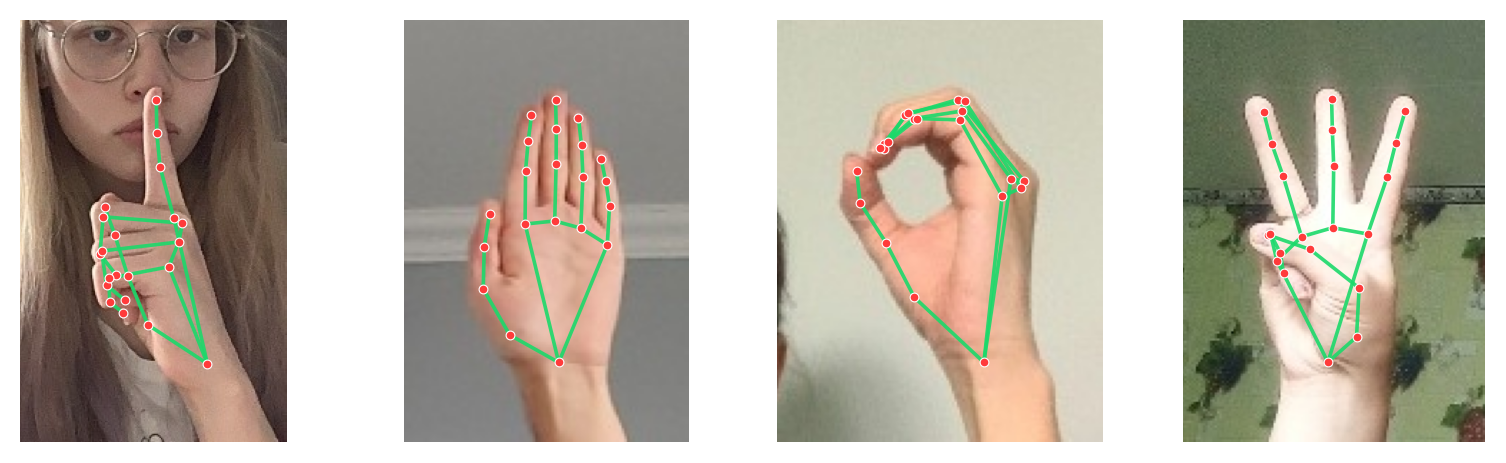
\includegraphics[width=\columnwidth]{figures/sample_inputs.png}
  \caption{Representative preprocessed inputs. Each panel shows a
  MediaPipe-cropped RGB hand (the image-branch input) with its 21 crop-relative
  landmarks overlaid as the MediaPipe skeleton (the landmark-branch input).
  Examples are drawn from \texttt{sample\_preprocessed\_outputs/}\evidence{DATA}.}
  \label{fig:sample-inputs}
\end{figure}

\begin{table}[t]
  \centering
  \caption{Processed split distribution reported by the team presentation.
  Counts reflect samples retained after preprocessing.}
  \label{tab:dataset}
  \scriptsize
  \setlength{\tabcolsep}{3.2pt}
  \begin{tabular}{lrrrrrrr}
    \toprule
    Split & N/A & fist & like & OK & one & palm & Total \\
    \midrule
    Train & 487094 & 21079 & 20421 & 21646 & 21267 & 22196 & 593703 \\
    Val.  & 58407  & 2669  & 2625  & 2816  & 2661  & 2804  & 71982 \\
    Test  & 99385  & 4602  & 4568  & 4808  & 4633  & 4784  & 122780 \\
    \bottomrule
  \end{tabular}
  \vspace{2pt}

  \raggedright\scriptsize Source: Team 14 presentation
  \evidence{PRES}. The original machine-readable count log was not committed.
\end{table}

Table~\ref{tab:dataset} shows a substantial imbalance: the N/A split is
approximately eight times the size of an individual target class
\evidence{PRES}. Phase 1 therefore uses inverse-frequency sampling, while
Phase 2 uses inverse-frequency loss weights.

\subsection{Landmark-synchronized augmentation}

The official test applies reasonable perturbations such as bounding-box
jitter and blur~\cite{courseSpec}. Training therefore applies
\result{$\pm10\%$}{AUG} crop jitter, Gaussian blur with
$\sigma\in\result{[0.1,1.5]}{AUG}$, brightness/contrast/saturation jitter of
\result{$\pm20\%$}{AUG}, horizontal flip with probability
\result{0.5}{AUG}, and rotation up to \result{$\pm15^\circ$}{AUG}. Spatial
changes update the landmarks together with the image. For example, rotation
around the crop center uses
\begin{align}
x' &= (x-.5)\cos\theta-(y-.5)\sin\theta+.5,\\
y' &= (x-.5)\sin\theta+(y-.5)\cos\theta+.5.
\end{align}
This prevents image-landmark disagreement during multimodal training.

\section{Training and Calibration}
\label{sec:training}

\subsection{Phase 1: image pretraining}

The first stage trains the image branch with a temporary
\result{$64{\to}6$}{P1} head for \result{20}{P1} epochs. We use Adam
~\cite{kingma2015adam} with learning rate \result{$10^{-3}$}{P1}, batch size
\result{256}{P1}, cross-entropy loss, and cosine annealing. A
\texttt{WeightedRandomSampler} assigns each class equal expected sampling
weight. The project progress record reports a best validation accuracy of
\result{86.15\%}{PROG}.

\subsection{Phase 2: joint optimization}

The best Phase-1 image weights initialize the full model. Joint training runs
for \result{30}{P2} epochs with batch size \result{256}{P2}. The pretrained
image branch uses learning rate \result{$10^{-4}$}{P2}, while the new landmark
and fusion layers use \result{$5\times10^{-4}$}{P2}. The loss uses
inverse-frequency class weights, with the N/A weight multiplied by
\result{1.5}{P2} to encourage conservative decisions. Checkpoints are selected
by validation contest score rather than accuracy alone. The reported best
validation accuracy is \result{96.75\%}{PROG}.

\subsection{Threshold calibration}

After training, softmax outputs for the validation set are cached and scored
over a \result{$14\times11=154$}{CAL} grid. Confidence thresholds span
\result{0.30--0.95}{CAL}; margin thresholds span
\result{0.00--0.50}{CAL}. Figure~\ref{fig:heatmap} shows that the best
validation contest score, \result{11,936}{HEAT}, occurs at the conservative
confidence threshold of 0.95.

\begin{figure}[t]
  \centering
  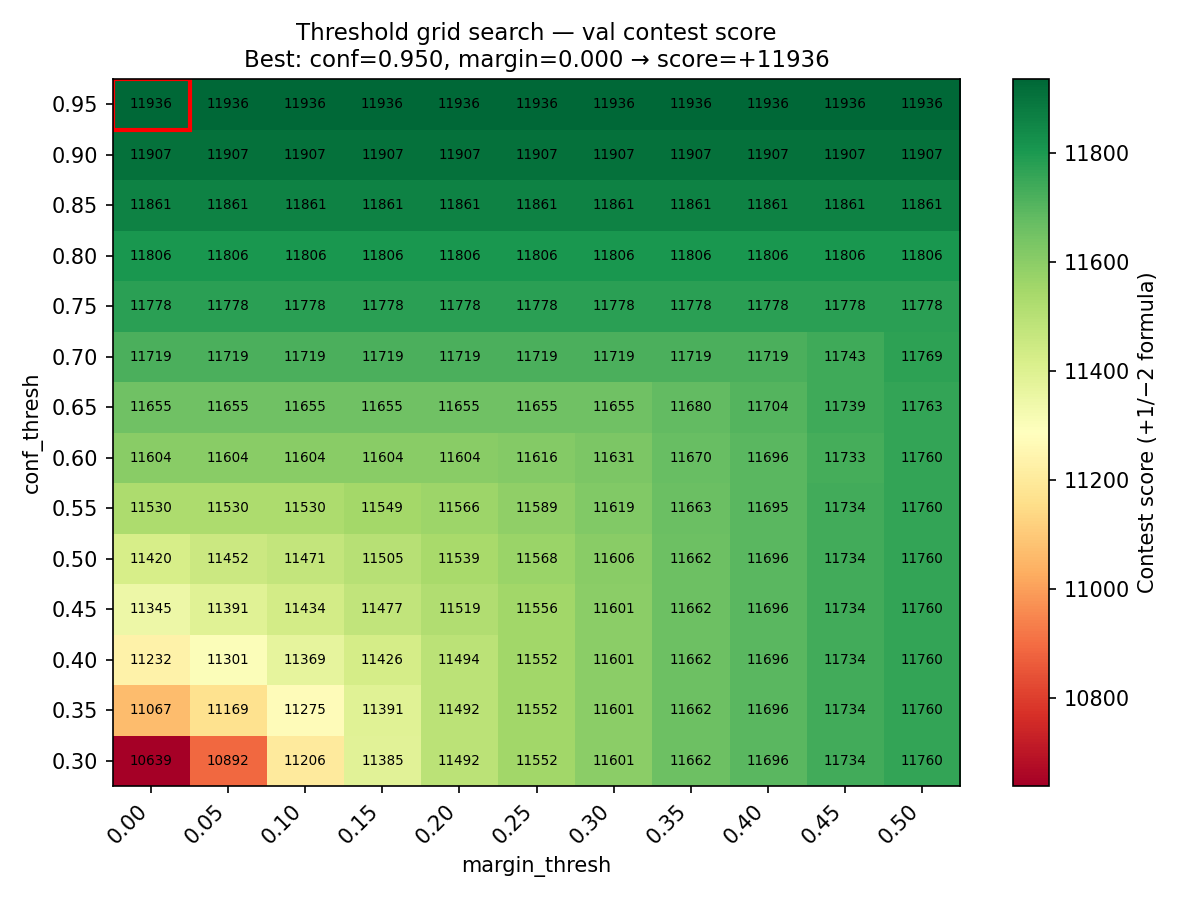
\includegraphics[width=\columnwidth]{figures/threshold_heatmap.png}
  \caption{Validation contest score over the calibration grid. Each cell
  applies one confidence-margin pair to the same cached validation
  probabilities and evaluates the official $+1/-2$ objective.}
  \label{fig:heatmap}
\end{figure}

\section{Results}
\label{sec:results}

\subsection{Validation and model size}

\begin{table}[t]
  \centering
  \caption{Training and calibration results reported by project artifacts.}
  \label{tab:training-results}
  \small
  \begin{tabular}{lcc}
    \toprule
    Stage & Validation accuracy & Contest score \\
    \midrule
    Image pretraining & 86.15\%\evidence{PROG} & -- \\
    Joint dual-stream & 96.75\%\evidence{PROG} & -- \\
    Calibrated model & -- & 11936\evidence{HEAT} \\
    \bottomrule
  \end{tabular}
\end{table}

The architecture contains \result{36,039}{VERIFY} trainable parameters. There
are two relevant size measurements. Summing model parameters and registered
buffers gives \result{0.142 MiB}{VERIFY}, the value shown in the architecture
slides. The serialized \texttt{weights.pt} file is
\result{176,372 bytes (0.168 MiB)}{VERIFY} because PyTorch serialization adds
metadata. The latter is consistent with the leaderboard model-size score of
\result{29.5/30}{PRES}. Distinguishing these quantities resolves the apparent
difference between the presentation's ``0.142 MB'' model statistic and the
submitted file size.

\subsection{Leaderboard performance}

\begin{table}[t]
  \centering
  \caption{Two official-evaluation runs reported in the presentation.
  ``Total'' is the subtotal before the 30-point presentation component.}
  \label{tab:leaderboard}
  \small
  \setlength{\tabcolsep}{4pt}
  \begin{tabular}{lrrrr}
    \toprule
    Run & Size & Basic & Robustness & Total / 90 \\
    \midrule
    1 & 29.5 & 19.4 & 32.5 & \textbf{81.4} \\
    2 & 29.5 & \textbf{20.0} & 31.0 & 80.5 \\
    \bottomrule
  \end{tabular}
  \vspace{2pt}

  \raggedright\scriptsize All values in this table are transcribed from the
  final presentation\evidence{PRES}.
\end{table}

Run 1 achieved the stronger overall subtotal because its 1.5-point robustness
advantage outweighed Run 2's 0.6-point basic-performance advantage. Run 2
reached the maximum reported basic-performance score, but the lower robustness
score suggests that model selection must account for real-world N/A examples
rather than relying only on the HaGRIDv2-derived test set.

\subsection{Baseline comparison: the N/A training distribution}
\label{sec:baseline}

To isolate how the N/A class should be constructed, we compare the submitted
model against an earlier team baseline\evidence{BASE} that shares the same
dual-stream concept---a CNN image branch, a landmark MLP, and a fused
classifier---but differs in two respects. First and most importantly, the
baseline draws its N/A training data from only five specific HaGRIDv2
categories (\texttt{dislike}, \texttt{peace}, \texttt{stop}, \texttt{call},
and \texttt{no\_gesture}), each capped at \result{4{,}000}{BASE} images,
whereas the submitted model treats \emph{every} retained non-command one-hand
category as N/A (about 487k training samples; Section~\ref{sec:data}). Second,
the baseline uses plain $3\times3$ convolutions on a $128\times128$ crop with a
single \result{0.60}{BASE} confidence threshold for rejection, instead of the
depthwise-separable blocks and multi-stage rejection of
Section~\ref{sec:method}.

\begin{table}[t]
  \centering
  \caption{Effect of the N/A training distribution. Both models use the same
  dual-stream concept and the official $+1/-2$ scoring; they differ mainly in
  how the N/A class is built. Submitted scores are from the
  presentation\evidence{PRES}; the baseline model and its scores are the team's
  earlier run\evidence{BASE}.}
  \label{tab:baseline}
  \small
  \setlength{\tabcolsep}{4pt}
  \begin{tabular}{@{}lp{0.34\columnwidth}rr@{}}
    \toprule
    Model & N/A training data & Basic\,/20 & Robust.\,/40 \\
    \midrule
    Submitted & all non-command one-hand poses ($\approx$487k)
              & \textbf{19.4} & \textbf{32.5} \\
    Baseline  & 5 categories, $\le$4k each ($\le$20k)
              & 7.6 & 5.0 \\
    \bottomrule
  \end{tabular}
\end{table}

Table~\ref{tab:baseline} reports both models under the official rule. The
narrow-N/A baseline scores only 7.6/20 on basic performance and 5.0/40 on
robustness, against 19.4 and 32.5 for the submitted model. The robustness gap
is the most telling: a classifier exposed to only five N/A gesture types in
training has no representation of the broad space of everyday hand poses in the
TA-shot interference set, so it false-triggers frequently---and under the
$+1/-2$ rule each false trigger is doubly costly. The two models also differ
architecturally, so this is a baseline comparison rather than a single-variable
ablation; nonetheless, the dominant cause of the gap is the N/A distribution.
Defining N/A as the full diversity of non-command poses, rather than a handful
of curated categories, is what makes the rejection behavior generalize to
real-world inputs, and it is the main reason the submitted model is
substantially more robust.

\subsection{Modality ablation}
\label{sec:modality}

To quantify each input stream's contribution, we trained a landmark-only
variant---the landmark branch followed by the same six-way head, with no image
branch---under the same Phase-2 training protocol\evidence{ABL}.
Table~\ref{tab:modality} places it beside the image-only Phase-1 model and the
full fusion model.

\begin{table}[t]
  \centering
  \caption{Modality ablation (best validation accuracy). Image-only and fusion
  are the original Phase-1/Phase-2 runs\evidence{PROG}; landmark-only is a
  dedicated run on a freshly re-preprocessed copy of the dataset under the same
  protocol\evidence{ABL}. The two data builds are not identical, so the
  landmark-only vs.\ fusion difference should be read as approximate.}
  \label{tab:modality}
  \small
  \setlength{\tabcolsep}{6pt}
  \begin{tabular}{lrr}
    \toprule
    Configuration & Params & Val.\ accuracy \\
    \midrule
    Image-only (Phase 1)        & 13{,}639 & 86.15\% \\
    Landmark-only               & 18{,}694 & 96.60\% \\
    Fusion (image $+$ landmark) & 36{,}039 & \textbf{96.75\%} \\
    \bottomrule
  \end{tabular}
\end{table}

The landmark-only model reaches \result{96.60\%}{ABL} validation accuracy with
only 18{,}694 parameters---close to the full fusion model
(\result{96.75\%}{PROG}) and far above the image-only model
(\result{86.15\%}{PROG}). Hand geometry therefore carries most of the
discriminative signal for these six classes on clean validation data. This
ablation was run only after the fusion model had been finalized and submitted,
on a freshly re-preprocessed copy of the dataset; the image-only and fusion
figures are from the original build, so the small landmark-only vs.\ fusion
accuracy gap should not be over-interpreted, although the large margin over
image-only is robust to that difference.

We nonetheless keep the image branch in the submitted model, for robustness
rather than clean-set accuracy. The landmark stream depends entirely on
MediaPipe's landmark estimates; when those degrade or fail---through occlusion,
motion blur, unusual viewpoints, or detection errors that are common in
real-world capture---a landmark-only classifier has no fallback, whereas the
image branch supplies an independent appearance-based signal that can still
yield a correct prediction. This is consistent with the evidence we do have:
the full model's best validation contest score
(\result{$+$11{,}539}{PROG}, default gates) exceeds the landmark-only model's
(\result{$+$11{,}233}{ABL}) by more than the small accuracy gap suggests,
indicating the image branch already helps on borderline cases under the
asymmetric scoring. A controlled real-world comparison of the two would
quantify this robustness benefit directly and remains future work.

\section{Discussion and Limitations}
\label{sec:discussion}

The results support three practical conclusions. First, a small custom network
is sufficient for a high challenge score: the submission uses less than
0.2 MiB of serialized weights while retaining strong target-set performance.
Second, calibration matters because the evaluation heavily penalizes false
activation. The selected threshold of 0.95 deliberately trades recall for
precision. Third, the baseline comparison in Section~\ref{sec:baseline} shows
that the N/A training distribution, not the network capacity, dominates
real-world robustness: replacing a few curated N/A categories with the full
diversity of non-command poses raises the robustness score from 5.0 to 32.5.
The remaining gap between basic and robustness scores still indicates a
residual domain shift between HaGRIDv2 imagery and TA-shot daily-action
examples.

The available evidence also has limitations. The repository contains the
training and calibration code, final weights, thresholds, and heatmap, but not
the original Phase-1/Phase-2 logs or per-example leaderboard predictions.
Consequently, the validation accuracies are traceable to the project progress
record, while the leaderboard table is traceable to the team presentation;
neither was independently recomputed in this report.
The modality ablation (Section~\ref{sec:modality}) shows that the landmark
stream alone nearly matches the full model, but image-only and landmark-only
were measured on slightly different data builds; a fully controlled
single-build ablation of all three configurations remains future work.
Finally,
latency and energy consumption were not measured on a specified edge device;
small model size alone does not establish real-time performance on every
deployment target.

\section{Reproducibility and Evidence}
\label{sec:evidence}

Table~\ref{tab:evidence-ledger} maps every evidence marker used beside a
quantitative claim to source code, a generated artifact, the official
specification, or the final presentation. The submitted report folder includes
the presentation PDF and a verification script for model statistics.

\begin{table*}[t]
  \centering
  \caption{Evidence ledger for implementation details and quantitative claims.}
  \label{tab:evidence-ledger}
  \small
  \begin{tabular}{>{\bfseries}p{0.08\textwidth}p{0.35\textwidth}p{0.49\textwidth}}
    \toprule
    Key & Authoritative source & Claims supported \\
    \midrule
    \phantomsection\label{ev:SPEC}SPEC
      & \texttt{source/Final\_Hand\_Gesture\_specs.pdf}; Ref.~\cite{courseSpec}
      & Inputs, class definitions, limits, scoring rules, and test composition. \\
    \phantomsection\label{ev:INFER}INFER
      & \codepath{inference.py}
      & Input normalization, label mapping, thresholds, and rejection logic. \\
    \phantomsection\label{ev:ARCH}ARCH
      & \codepath{model/architecture.py}
      & Layer dimensions, feature dimensions, and dropout. \\
    \phantomsection\label{ev:AUG}AUG
      & \codepath{train/augment.py}; \codepath{train/dataset.py}
      & Augmentation types, probabilities, and parameter ranges. \\
    \phantomsection\label{ev:P1}P1
      & \codepath{train/train_phase1.py}
      & Phase-1 architecture and hyperparameters. \\
    \phantomsection\label{ev:P2}P2
      & \codepath{train/train_phase2.py}
      & Phase-2 optimization, loss weighting, and checkpoint selection. \\
    \phantomsection\label{ev:CAL}CAL
      & \codepath{train/calibrate.py}; \codepath{model/thresholds.json}
      & Grid definition and deployed thresholds. \\
    \phantomsection\label{ev:HEAT}HEAT
      & \texttt{figures/threshold\_heatmap.png};
        \codepath{train/plot_threshold_heatmap.py}
      & Grid-search scores and selected calibration point. \\
    \phantomsection\label{ev:VERIFY}VERIFY
      & \texttt{evidence/verify\_report\_numbers.py};
        \texttt{evidence/compute\_flops.py};
        \codepath{model/architecture.py}; \codepath{model/weights.pt}
      & Parameter count, per-branch parameters, tensor footprint, checkpoint
        size, computed size score, and the MAC/FLOP inference cost. \\
    \phantomsection\label{ev:DATA}DATA
      & \codepath{download_and_preprocess.py};
        \codepath{hand_preprocess.py};
        \texttt{figures/make\_sample\_inputs.py};
        \texttt{sample\_preprocessed\_outputs/}
      & Dataset source, label mapping, exclusion policy, preprocessing, and the
        rendered sample-input figure. \\
    \phantomsection\label{ev:BASE}BASE
      & \texttt{evidence/baseline/}: \texttt{download\_dataset.sh},
        \texttt{subsample\_dataset.py}, \texttt{baseline\_inference.py}
      & Baseline N/A category selection, the 4{,}000-per-class cap, baseline
        architecture and 0.60 threshold, and its leaderboard scores
        (team-reported; raw export not committed). \\
    \phantomsection\label{ev:ABL}ABL
      & \codepath{train/ablation_landmark_only.py}
      & Landmark-only ablation: model definition, parameter count, and its best
        validation accuracy and contest score (run on a re-preprocessed copy of
        the dataset under the Phase-2 protocol). \\
    \phantomsection\label{ev:PROG}PROG
      & \codepath{PROGRESS.md}
      & Recorded Phase-1 and Phase-2 validation accuracies and the selected
        training run. Original training logs are not present in the repository. \\
    \phantomsection\label{ev:PRES}PRES
      & \texttt{source/Hand Gesture Classification on Edge Devices.pdf};
        Ref.~\cite{team14presentation}
      & Retained split counts and leaderboard results. The original evaluation
        export or screenshot is not present in the repository. \\
    \bottomrule
  \end{tabular}
\end{table*}

\section{Conclusion}
\label{sec:conclusion}

We developed a compact dual-stream hand-gesture classifier that combines RGB
appearance with MediaPipe landmark geometry and uses calibrated rejection to
address asymmetric false-trigger costs. The final submission contains only
36,039 trainable parameters, and its strongest reported leaderboard run scored
81.4 out of 90 before presentation points. The remaining performance gap is
primarily in real-world robustness, motivating future work on hard-negative
collection, explicit modality ablation, and evaluation on measured edge
hardware.

\section*{Code Availability}

The complete inference and training source code, final model weights, threshold
configuration, and environment requirements are available at
\url{\ProjectRepository}. The report package includes the exact presentation,
specification, figures, and verification helper used to support its claims.

\FloatBarrier

% Main text, including the evidence ledger, ends here. References and the
% contribution table below are excluded from the 10-page main-text limit.
\MainTextEndsHere

\bibliographystyle{IEEEtran}
\bibliography{references}

\clearpage
\onecolumn
\section*{Team Member Contributions}

\begin{table}[h!]
  \centering
  \caption{Team member contribution statement.}
  \label{tab:contributions}
  \small
  \begin{tabular}{p{0.16\textwidth}p{0.16\textwidth}p{0.60\textwidth}}
    \toprule
    Member & Student ID & Specific contributions \\
    \midrule
    {\zhfont 王昱閔} & 112062114
      & Model architecture design; model training and hyperparameter tuning;
        presentation; report writing. \\
    {\zhfont 王辰竹} & 112062105
      & Hyperparameter tuning; presentation. \\
    {\zhfont 羅詠璿} & 112060002
      & Baseline model training; real-time demo; report writing. \\
    \bottomrule
  \end{tabular}
\end{table}

\end{document}
